\documentclass{ecnreport}

\stud{Master 1 CORO / Option Robotique}
\topic{Robot Operating System}
\author{G. Garcia, O. Kermorgant}

\begin{document}

\inserttitle{Robot Operating System}

\insertsubtitle{Lab 1: Packages, launch files,  parameters and topic remapping}

\section{Goals}

In this lab we will create a launcher that launches three nodes:

\begin{itemize}
 \item one (\texttt{capture\_key\_node}) for capturing keystrokes  from the keyboard and publish it in ROS.
\item  the other two (\texttt{move\_joint\_node}) that subscribe to the same type of topic published by the \texttt{capture\_key\_node},
moving each one a predefined articulation of the robot defined by parameter.
The keys used to increment and decrement the position as well as the increment value are defined by parameters  in each node \texttt{move\_joint\_node}.
\end{itemize}

\section{Deliverables}

\begin{itemize}
 \item A text file with the answers to the questions of this sheet
 \item The launch files of the first task
\end{itemize}
Files should be zipped and sent by mail (G. Garcia) or through the lab upload form (O. Kermorgant).

\begin{figure}[h]\centering
 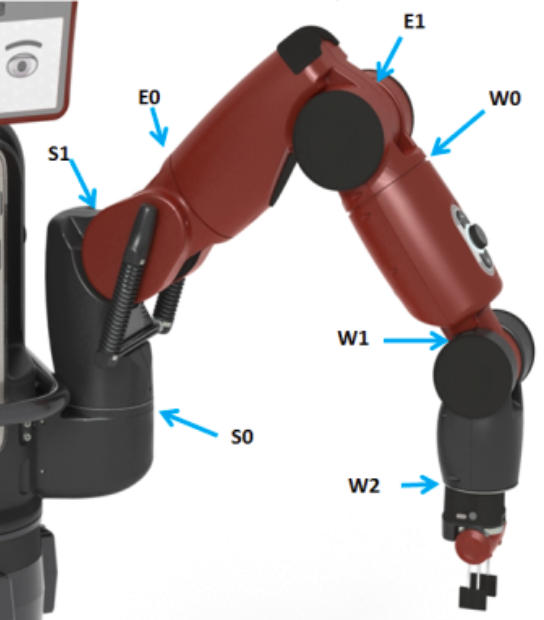
\includegraphics[width=.3\linewidth]{baxter} \\
  \begin{tabular}{|c|c|c|c|c|c|c|c|}
  \hline
  group & 1 & 2 & 3 & 4 & 5 & 6 & 7 \\\hline
  joints (\texttt{left\_} \& \texttt{right\_})& \texttt{s0} & \texttt{s1}& \texttt{e0} & \texttt{e1} & \texttt{w0} & \texttt{w1} & \texttt{w2} \\\hline
 \end{tabular}
 \caption{Baxter joints}
 \label{baxter}
\end{figure}
\section{Specification of the robot and available packages}

The Baxter robot has $2\times 7$ joints as shown in \Fig{baxter}, the names of which are listed in the table.
The goal is to have each group control 2 of the joints through the same topic.

\subsection{Available packages}

Two packages are included in this lab:
\begin{itemize}
 \item \texttt{capture\_key} contains a single node (\texttt{capture\_key\_node}) that:
 \begin{itemize}
  \item Captures the keystrokes
  \item Publishes their ASCII code on the \texttt{/key\_typed} topic
  \item Does not subscribe to any topic
 \end{itemize}
 \item \texttt{move\_joint} contains a single node (\texttt{move\_joint\_node}) that:
 \begin{itemize}
  \item Moves the joint of a robot in position mode, incremening or decrementing it according to the key which as been typed.
  \item Subscribes to:
  \begin{itemize}
   \item \texttt{/key\_hit} as topic for the incoming key strokes
   \item \texttt{/robot/joint\_states} for the current state variables of the robot
  \end{itemize}
  \item Publishes a joint command for the controlled joint, to the topic \texttt{/joint\_command}
  \item Has the following parameters:
  \begin{itemize}
   \item \texttt{joint\_name} to tell the joint to be controlled. This parameter is mandatory and does not have a default value.
   \item \texttt{incr\_key} for the increment key (default +, ASCII code 43)
   \item \texttt{decr\_key} for the increment key (default -, ASCII code 45)
  \end{itemize}
 \end{itemize}
\end{itemize}

\section{Using launch files}

Tutorials on how to use launch files can be found on internet. These files allow running several nodes in a single command.

Create a launch file to control two of the joints of the Baxter robot (1 \texttt{capture\_key\_node} + 2 \texttt{move\_joint\_node}), according to the table
and your group number. The contributions of all groups will allow controlling most of the joints. 

\subsection{First launch file attempt}

For this launch; the \texttt{<node ... /node>} sections should be minimal: no node renaming, no remapping.

\begin{itemize}
 \item What happens when this is launched from only one computer?
 \item What happens when this is launched from several computers?
 \item Coordinate with other groups to have nodes with different names.
 \item Coordinate with other groups to have nodes in different namespaces (use the \texttt{group} tag).
\end{itemize}

\subsection{Second launch file attempt}

What is the behavior of the current launch file? Explain how to solve the issue (at this point poor Baxter has not moved yet).

\subsection{Third launch file attempt}

Now modify the launch file so that topics are remapped and Baxter actually moves accordingly to each group's typed keys.


 




\end{document}
